\documentclass[12pt, a4paper, oneside]{ctexart}
\usepackage{amsmath, amsthm, amssymb, bm, color, graphicx, geometry, hyperref, mathrsfs,extarrows, braket, booktabs, array}

\linespread{1.5}
%\geometry{left=2.54cm,right=2.54cm,top=3.18cm,bottom=3.18cm}
\geometry{left=1.84cm,right=1.84cm,top=2.18cm,bottom=2.18cm}
\newenvironment{problem}{\par\noindent\textbf{题目. }}{\bigskip\par}
\newenvironment{solution}{\par\noindent\textbf{解答. }}{\bigskip\par}
\newenvironment{note}{\par\noindent\textbf{注记. }}{\bigskip\par}

% 基本信息
\newcommand{\RQ}{\today} % 日期
\newcommand{\km}{实变函数} % 科目
\newcommand{\bj}{强基数学002} % 班级
\newcommand{\xm}{吴天阳} % 姓名
\newcommand{\xh}{2204210460} % 学号
\newcommand{\XH}{59} % 序号

\begin{document}

%\pagestyle{empty}
\pagestyle{plain}
\vspace*{-15ex}
\centerline{\begin{tabular}{*6{c}}
    \parbox[t]{0.25\linewidth}{\begin{center}\textbf{日期}\\ \large \textcolor{blue}{\RQ}\end{center}} 
    & \parbox[t]{0.15\linewidth}{\begin{center}\textbf{科目}\\ \large \textcolor{blue}{\km}\end{center}}
    & \parbox[t]{0.2\linewidth}{\begin{center}\textbf{班级}\\ \large \textcolor{blue}{\bj}\end{center}}
    & \parbox[t]{0.1\linewidth}{\begin{center}\textbf{姓名}\\ \large \textcolor{blue}{\xm}\end{center}}
    & \parbox[t]{0.15\linewidth}{\begin{center}\textbf{学号}\\ \large \textcolor{blue}{\xh}\end{center}}
    & \parbox[t]{0.1\linewidth}{\begin{center}\textbf{序号}\\ \large \textcolor{blue}{\XH}\end{center}} \\ \hline
\end{tabular}}
\vspace*{4ex}

\def\P{\mathbf{P}}
\def\R{\mathbf{R}}
\paragraph{习题 2.2}
\paragraph{2.}设$\P'$为直线上的开区间全体,作$\P'$上的集函数$m'$如下:$m'((\alpha,\beta))=\beta-\alpha$,证明$m'$必可唯一地延拓成$\R(\P')$上的测度。
\begin{solution}
    由题可知$\P = \{(a,b):-\infty\leqslant a<b\leqslant +\infty\}$,则对于$\forall -\infty < a \leqslant b < +\infty$,有
    \begin{equation*}
        \begin{aligned}
            (-\infty,+\infty) - (-\infty, a) =&\ [a,+\infty)\in \R(\P')\\
            (-\infty, +\infty) - (b,+\infty) = &\ (-\infty, b]\in \R(\P')\\
            [a,+\infty)\cap (-\infty, b] =&\ [a,b]\in \R(\P')
        \end{aligned}
    \end{equation*}
    则$\R(\P')$包含直线上一切区间和单点,对任意的$E\in \R(\P')$,可以分解为不交的开区间和单点的并集,即
    \begin{equation*}
        E = \left(\bigcup_{i=1}^n(a_i,b_i)\right)\cup\{c_1,c_2,\cdots, c_m\}
    \end{equation*}
    令$m'$在$\R(\P')$上的测度为
    \begin{equation*}
        m'(E) = \sum_{i=1}^m((a_i,b_i)) + \sum_{j=1}^mm'(\{c_j\})
    \end{equation*}
    下证$m'$在单点的测度为$0$,才能使得$m'(E)$具有唯一性,对于$(a,b)$上的任意的分解,将分解的开区间端点从小到大排序
    \begin{equation*}
        a=a_1<b_1=a_2<b_2=\cdots =a_m<b_m=b
    \end{equation*}
    则$b-a=m'((a,b)) = \sum_{i=1}^m(b_i-a_i)+\sum_{j=1}^mm'(\{c_j\}) = b-a +\sum_{j=1}^mm'(\{c_j\})$,则$m'(\{c_j\})=0$,由于单点可以任意添加在区间$(a,b)$中,且$a,b$具有任意性,则$\forall x\in\mathbb{R}, m'(x) = 0$,且可以类比于$m$是$\R_0$上的测度,证明$m'$在$\R(\P')$上是单值的,则$m'$具有唯一性,再类比地证明$m'$在$\R(\P')$上是可列可加的,即可证明$m'$是$\R(\P')$上的测度。
\end{solution}
\paragraph{4.}设$\mu$是直线上环$\R_0$上的测度。证明:存在单调增加右连续的函数$g(x)$,使得$\mu(E)  = \mu_g(E)(e\in\R_0)$的充要条件是对一切$(a,b]\in \P,\mu((a,b])<\infty.$(此即说明:对$\P$中每个集都有限的$\R_0$上测度必是$g$测度)
\begin{proof}
    “$\Rightarrow$”:反设$\exists(a, b]\in \P$,使得$\mu((a, b]) = \infty$,则$\mu_g((a,b]) = g(b)-  g(a) = \infty$,所以$g(b) = \infty$,则$g$函数在$b$处发散到$\infty$,与$g(b)$处右连续矛盾。

    “$\Leftarrow$”:令$g(x) = \mu(-\infty,x]$,$\forall \varepsilon > 0,\ \exists \delta = \varepsilon$,使得$\forall y  \in(x,x+\delta)$,有$g(y)-g(x)\leqslant \mu((x,x+\delta]) = \delta = \varepsilon$,则$g$函数在$x$处右连续。

    由$\mu$具有非负性,则$\forall y > x$,由$g(y) - g(x) = \mu((x, y]) > 0$,则$g(y) > g(x)$,所以$g$函数单调增加。
\end{proof}
\paragraph{6.}设$\{\mu_n\}$是环$\R$上一列测度,并且对一切$E\in\R$,以及任何自然数$n$,都有$\mu_n(E)\leqslant 1.$证明
\begin{equation*}
    \mu(E) = \sum_{n=1}^{\infty}\frac{1}{2^n}\mu_n(E)\quad(E\in\R),
\end{equation*}
也是$\R$上测度,并且满足$\mu(E)\leqslant 1,\ (E\in \R)$。

\begin{proof}
    令$E=\varnothing$,则$\mu_n(\varnothing) = 0\ (n \geqslant 1)$,所以$\mu(\varnothing) = \sum_{n=1}^\infty\frac{1}{2^n}\mu_n(\varnothing) = 0$。
    
    由非负性可知$E\in \R$,有$\mu_n(E)\geqslant 0$,所以$\mu(E) = \sum_{n=1}^{\infty}\frac{1}{2^n}\mu_n(E)\geqslant 0$。

    令$E = \bigcup\limits_{i=1}^\infty E_i$,$E_i$互不相交,则$\mu(E_i)=\sum_{n=1}^\infty\frac{1}{2^n}\mu_n(E_i)$,由$\mu_n$的可列可加性有,$\mu_n(E) = \sum_{i=1}^\infty\mu_n(E_i)$,则
    \begin{equation*}
        \mu(E) = \sum_{n=1}^\infty\frac{1}{2^n}\mu_n\left(\bigcup_{i=1}^\infty E_i\right) = \sum_{n=1}^\infty\sum_{i=1}^\infty\frac{1}{2^n}\mu_n(E_i)\xlongequal[\text{可交换求和顺序}]{\text{正项级数}}\sum_{i=1}^\infty\sum_{n=1}^\infty\frac{1}{2^n}\mu_n(E_i) = \sum_{i=1}^\infty\mu(E_i)
    \end{equation*}
    
    由于$\mu_n(E)\leqslant 1$,所以$\displaystyle\mu(E) = \sum_{n=1}^{\infty}\frac{1}{2^n}\mu_n(E)\leqslant \sum_{n=1}^{\infty}\frac{1}{2^n} = 1$,则$\mu(E)\leqslant 1$。
\end{proof}
\paragraph{9.}设$\R_n(n=1,2,3,\cdots)$是集$X$上一列环,并且$\R_1\subset\R_2\subset\cdots\subset\R_n\subset\cdots.$又设$\mu_n$是$\R_n$上的测度,并且对任何$E\in \R_n$,当$m\geqslant n$时,$\mu_m(E)=\mu_n(E)$(通常称为$\{\mu_n\}$在$\{\R_n\}$上是\textbf{符合}的)。证明 (i) $\R=\bigcup\limits_{i=1}^{\infty}\R_n$是$X$上的环。(ii) 定义$\R$上函数$\mu$:对每个$E\in \R$,必存在某个$n$,$E\in\R_n$,规定$\mu(E)=\mu_n(E)$,证明$\mu$是$\R$上非负、空集上取值为$0$的有限可加集函数($\mu$未必是$\R$上测度,参见下面习题$10$)
\begin{proof}
    (i) 由于$\{\R_n\}$是单增的,所以$\R = \bigcup\limits_{n=1}^\infty \R_n = \lim\limits_{n\rightarrow \infty} \R_n$,由于$R_n$均为环,所以$\R$也是环。

    (ii) $\forall E\in \R$,$\exists n$使得$E\in \R_n$,则$\mu(E) = \mu_n(E)\geqslant 0$,由于$\varnothing\in\R_1$,则$\mu(\varnothing) = \mu_1(\varnothing) = 0$,对于任意有限长的集列$\{E_1,E_2,\cdots,E_n\}$,令$E_i\in \R_{n_i}$,取$M=\max\limits_{1\leqslant i\leqslant n}\{n_i\}$,则
    \begin{equation*}
        \mu\left(\bigcup_{i=1}^nE_i\right) = \mu_M\left(\bigcup_{i=1}^nE_i\right) = \sum_{i=1}^n\mu_M(E_i) = \sum_{i=1}^n\mu(E_i)
    \end{equation*}
    所以$\mu$具有有限可加性。
\end{proof}
\def\disp{\displaystyle}
\paragraph{10.}设$\displaystyle X=\{x:x=(x_1,x_2,\cdots, x_n,\cdots),x_n=\frac{j}{n^2}(j=0,1,2,\cdots,n^2),\sum\limits_{n=1}^{\infty}x_n^{\frac{1}{2}}<\infty\}$,对每个自然数$n$,$x\in X$,令$\widetilde{x}_n = \{y:y\in X, y_1=x_1,\cdots,y_n=x_n\}$(即$\widetilde{x}_n$是$X$中一切前$n$个坐标与$x$相同的$y$全体所成的集),$\R_n$是由一切$\widetilde{x}_n$张成的环(显然,$\R_n$是有限集)。又在$\R_n$上作$\mu_n$如下,对任何$E\in\R_n$,如果$\displaystyle E=\bigcup\limits_{l=1}^k\widetilde{x}_n^{(l)},x_n^{(l)}\cap x_n^{(m)}=\varnothing(m\neq l)$,那么规定$\displaystyle \mu_n(E) = k\prod\limits_{j=1}^n\dfrac{1}{1+j^2}$,再规定$\mu_n(\varnothing) = 0$。证明:

(i) $\R_1\subset \R_2\subset \cdots\subset \R_n\subset \cdots$,并且$X\in\R_n(n=1,2,3,\cdots)$。

(ii) $\mu_n$是$\R_n$上测度,$\mu_n(X)=1$并且$\{\mu_n\}$在$\{\R_n\}$上是符合的(见习题9)。

(iii) 对每个自然数$n$,令$E_n=\{x:x=(x_1,\cdots,x_n,\cdots),0<x_i\leqslant 1,i=1,2,\cdots,n\}$,那么$E_1\supset E_2\supset \cdots\supset E_n\supset \cdots$,$\displaystyle \mu(E_n)=\prod\limits_{j=1}^n\left(1-\dfrac{1}{1+j^2}\right)$,$\lim\limits_{n\rightarrow \infty}\mu(E_n)\neq 0$,但是$\displaystyle\bigcap\limits_{n=1}^\infty E_n = \varnothing$。
\def\wtd{\widetilde}
\begin{proof}
(i) $\forall 1\leqslant n \leqslant m$,有$\disp \wtd{x}_n = \bigcup\{\wtd{y}_m:y\in X, y_1=x_1,\cdots,y_n=x_n\}$,则$\wtd{x}_n\in \R_m$,由$n, m$的任意性可知
\begin{equation*}
    R_1\subset R-2\subset \cdots \subset \R_n\subset \cdots
\end{equation*}

令$x^{(0)} = (0, x_2, x_3,\cdots),\ x^{(1)} = (1, x_2, x_3,\cdots)$,则$X = \wtd{x}_1^{(0)}\cup\wtd{x}_1^{(1)}$,所以$X\in \R_1$,则$X\in\R_n\ (n=1,2,\cdots)$。

(ii) 根据$\mu_n$的定义可知,$\mu_n$具有非负性,且空集取值为零,由于$\R_n$为有限集,所以只需证明可列可加性,令$\disp E = \bigcup_{l=1}^k\wtd{x}_n^{(l)}\in \R_n,x_n^{(l)}\cap x_n^{(m)} = \varnothing(m\neq l)$,则
\begin{equation*}
    \mu_n(E) = \mu_n\left(\bigcup_{l=1}^k\wtd{x}_n^{(l)}\right) = k\prod_{j=1}^n\frac{1}{1+j^2}=\sum_{l=1}^k\prod_{j=1}^n\frac{1}{1+j^2}=\sum_{l=1}^k\mu_n(\{\wtd{x}_n^{(l)}\})
\end{equation*}

下证$\{\mu_n\}$在$\{\R_n\}$上是符合的,设$E =  \bigcup_{l=1}^k\wtd{x}_n^{(l)}\in \R_n$,$\forall 1\leqslant n\leqslant m$,由于
\begin{equation*}
    \wtd{x}_n= \bigcup\{\wtd{y}_m:y\in X,y_1 = x_1,\cdots, y_n = x_n\} = \bigcup_{l=1}^M\wtd{y}_m^{(l)}
\end{equation*}
其中$\disp M = \prod_{i=n+1}^m(i^2+1)$,是由于$y$的$y_{n+1}, y_{n+2}, \cdots, y_m$具有任意性,总共有$M$中选择,则
\begin{equation*}
    \mu_m(E) = k\cdot M\prod_{j=1}^m\frac{1}{1+j^2} = k\cdot \prod_{i=n+1}^m(i^2+1)\prod_{j=1}^m\frac{1}{1+j^2} = k\cdot \prod_{j=1}^n\frac{1}{1+j^2} = \mu_n(E)
\end{equation*}
所以$\{\mu_n\}$在$\{\R_n\}$上是符合的,由(i)可知$X = \wtd{x}_1^{(0)}\cup\wtd{x}_1^{(1)}$,所以$\disp \mu_1(X) = 2\cdot\prod_{j=1}^n\frac{1}{1+j^2} = 1$,由于$\{\mu_n\}$在$\{\R_n\}$上是符合的,所以$\mu_n(X) = 1\ (n = 1,2,3,\cdots)$。

(iii) 由于$\disp E_n = \{x:x=(x_1,x_2,\cdots,x_n,\cdots),0<x_i\leqslant 1,i=1,\cdots, n\}=\bigcup_{l=1}^Mx_n^{(l)}$,其中$\disp M = \prod_{i=1}^ni^2$,则
\begin{equation*}
    \mu(E_n) = \mu_n(E_n) = M\prod_{j=1}^n\frac{1}{1+j^2} = \prod_{i=1}^ni^2\prod_{j=1}^n\frac{1}{1+j^2} = \prod_{j=1}^n\frac{j^2}{1+j^2} = \prod_{j=1}^n\left(1-\frac{1}{1+j^2}\right)
\end{equation*}
所以,$\disp \lim_{n\rightarrow\infty}\mu(E_n)=\lim_{n\rightarrow\infty}\prod_{j=1}^n\left(1-\frac{1}{1+j^2}\right)\neq 0$,由于
\begin{equation*}
    \begin{aligned}
        E_n=&\ \{x:(x_1,\cdots,x_n,\cdots),0 < x_i\leqslant 1,i=1,\cdots,n\}\\
        =&\ \left\{x:(x_1,\cdots,x_n,\cdots),x_n=\frac{j}{n^2}\ (j=1,2,\cdots, n^2),\ \sum_{n=1}^\infty x^{\frac{1}{2}}_n < \infty\right\}
    \end{aligned}
\end{equation*}

假设$\lim\limits_{n\rightarrow \infty}E_n\neq \varnothing$,则对于充分大的$n$,$\disp\exists x\in E_n$,令$\disp x = (\frac{j_1}{1^2},\cdots,\frac{j_n}{n^2},\cdots)$,有
\begin{equation*}
    \sum_{i=1}^\infty x_i^{\frac{1}{2}}\geqslant \sum_{i=1}^nx_i^{\frac{1}{2}} = \sum_{i=1}^n\frac{\sqrt{j_i}}{i}\geqslant \sum_{i=1}^n\frac{1}{i}
\end{equation*}
由于$\disp\sum_{i=1}^{\infty}\frac{1}{i}$发散,则当$n\rightarrow \infty$时,$\disp \sum_{i=1}^\infty x_i^{\frac{1}{2}}\geqslant \infty$,与$\disp \sum_{i=1}^\infty x_i^{\frac{1}{2}}<\infty$矛盾,所以$\disp\bigcap_{n=1}^\infty E_n=\lim_{n\rightarrow \infty}E_n = \varnothing$。

\end{proof}
\iffalse
% 图片模板
\centerline{
    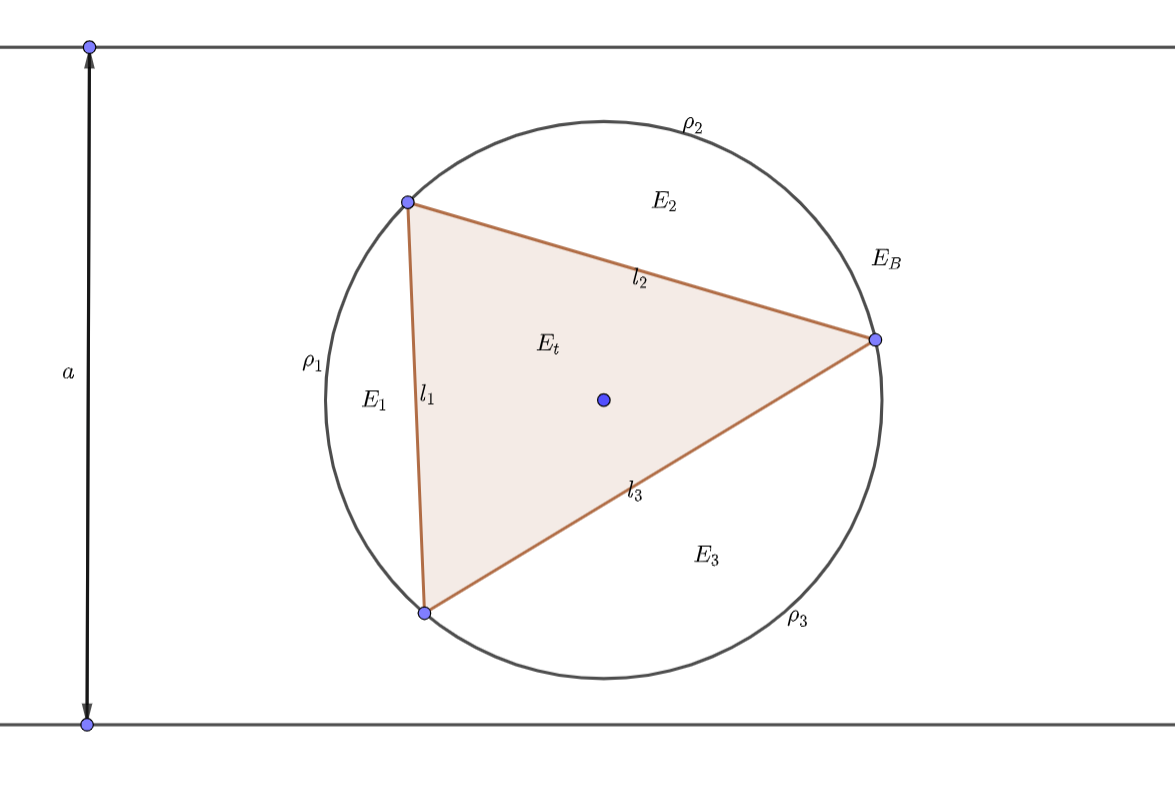
\includegraphics[width=0.8\textwidth]{figure.png}
}
\fi
\iffalse
% 表格模板
\renewcommand\arraystretch{0.8} % 设置表格高度为原来的0.8倍
\begin{table}[!htbp] % table标准
    \centering % 表格居中
    \begin{tabular}{p{1cm}<{\centering}p{1cm}<{\centering}p{3cm}<{\centering}p{5cm}<{\centering}} % 设置表格宽度
    %\begin{tabular}{cccc}
        \toprule
        $x_i$ & $f[x_1]$ & $f[x_i,x_{i+1}]$ & $f[x_i,x_{i+1},x_{i+2}]$ \\
        \midrule
        $x_0$ & $f(x_0)$ &                  &                          \\
        $x_0$ & $f(x_0)$ & $f'(x_0)$        &                          \\
        $x_0$ & $f(x_1)$ & $\frac{f(x_1)-f(x_0)}{x_1-x_0}$ & $\frac{f(x_1)-f(x_0)}{(x_1-x_0)^2}-\frac{f'(x_0)}{x_1-x_0}$\\
        \bottomrule
    \end{tabular}
\end{table}

\def\Log{\text{Log}} % 一个简单的宏定义
$\Log$ % 调用方法
\fi

\end{document}